\subsection{ソフトウェアエンジニアリング運用の基礎}

\subsubsection{ソフトウェアエンジニアリング運用の定義}

ソフトウェアエンジニアリング運用とは、ソフトウェア製品、情報技術インフラ、システムソフトウェア、アプリケーションソフトウェアが、開発中、保守中、実運用中に適切に動作するように使われる知識、技能、プロセス、ツールの総体である。

運用担当技術者は、単にサーバを見張る人ではない。コンテナや仮想サーバの準備、配備、設定、支援を行う。必要な環境をオンデマンドで提供し、継続的インテグレーション、試験、配備、監視をサービスとして提供する。障害を診断し、問題と解決策を記録し、優先順位を付け、影響を評価する。さらに、セキュリティ、データ保護、フェイルオーバー、容量、ストレージ、データベース性能、技術仕様書の整備にも関わる。

\par\smallskip\noindent\refstepcounter{table}\label{tab:ch06-02}\textbf{表 \thetable: 第06章 ソフトウェアエンジニアリング運用 表02}\par\smallskip
\begin{longtable}{L{45mm}L{105mm}}
\toprule
役割 & 主な責任 \\
\midrule
運用担当技術者 & 運用サービスを設計し、配備、監視、容量管理、障害対応、セキュリティ、復旧を実行または自動化する。 \\
ソフトウェア技術者 & 運用担当技術者が提供する運用サービスを使い、自分のソフトウェアを配備、監視、改善する。 \\
プラットフォーム技術者 & 開発者が自律的に使える共通基盤、セルフサービス環境、配備基盤、監視基盤を作る。 \\
SRE技術者 & 可用性、性能、遅延、容量、緊急対応、変更管理を、測定と自動化に基づいて改善する。 \\
\bottomrule
\end{longtable}

\subsubsection{ソフトウェアエンジニアリング運用プロセス}

運用プロセスは、既存のソフトウェアシステムまたは製品を配備、設定、運用、支援し、その完全性を保つための活動である。国際標準では、運用の準備、運用の実行、運用結果の管理、利用者支援が重要な活動として扱われる。

SWEBOK 06章では、運用活動を学習しやすくするため、次の三つのプロセス群として整理できる。

\par\smallskip\noindent\refstepcounter{table}\label{tab:ch06-03}\textbf{表 \thetable: 第06章 ソフトウェアエンジニアリング運用 表03}\par\smallskip
\begin{longtable}{L{35mm}L{115mm}}
\toprule
プロセス群 & 含まれる活動 \\
\midrule
運用計画 & 運用計画、供給者管理、開発環境と運用環境、可用性、継続性、サービス水準、容量、バックアップ、災害復旧、フェイルオーバー、安全性とセキュリティを扱う。 \\
運用提供 & 運用テスト、検証、受け入れ、配備、リリース、ロールバック、データ移行、問題解決を扱う。 \\
運用制御 & インシデント管理、変更管理、監視、測定、追跡、レビュー、運用支援、サービス報告を扱う。 \\
\bottomrule
\end{longtable}

\begin{figure}[htbp]
\centering
\IfFileExists{assets/generated_figures/ch06/fig-ch06-02.png}{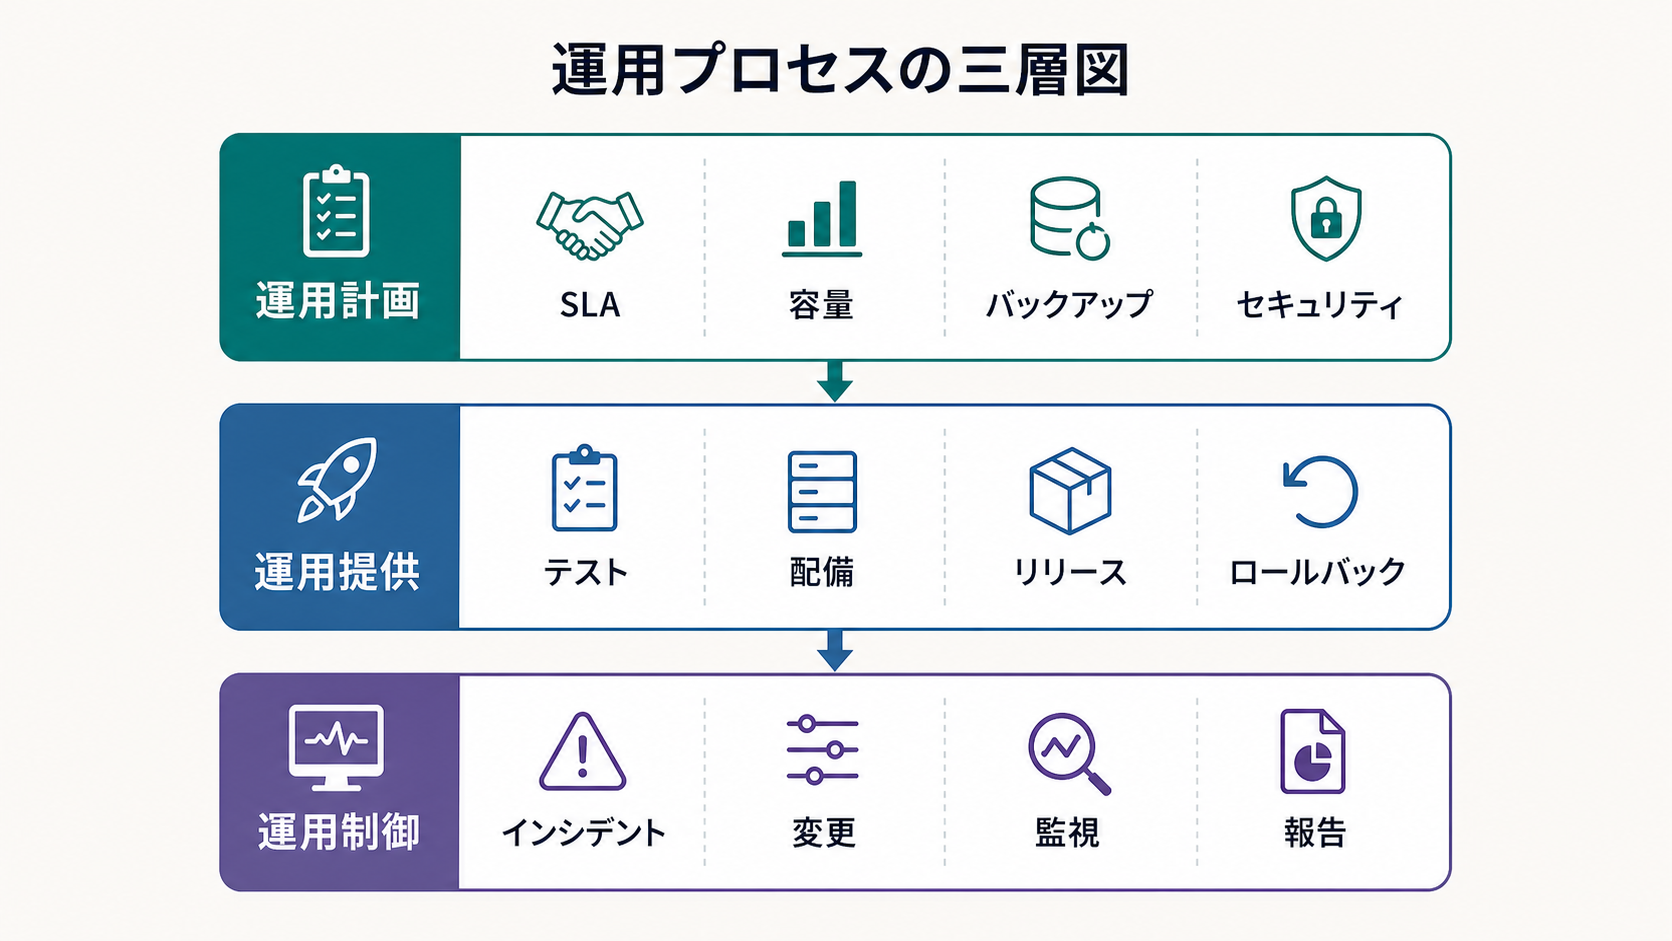
\includegraphics[width=0.96\linewidth]{assets/generated_figures/ch06/fig-ch06-02.png}}{\fbox{\parbox[c][48mm][c]{0.9\linewidth}{\centering 画像生成待ち\\運用プロセスの三層図}}}
\caption{運用プロセスの三層図}
\label{fig:ch06-02}
\end{figure}

\subsubsection{ソフトウェア導入}

ソフトウェア導入とは、ソフトウェアまたは更新版を利用者に使える状態にするため、対象環境に配置し、設定し、確認する作業である。導入では、旧版の削除、対象環境に合わせた設定、必要なディレクトリ、登録情報、環境変数の作成などが行われる。多くの場合、これらはスクリプトで実行される。

組込みシステムでは、電子的な配布だけでなく、物理媒体を使うこともある。いずれの場合でも、導入後には検証が必要である。導入が成功したか、必要なファイルが配置されたか、設定が正しいか、最低限の動作確認ができるかを確認する。

\subsubsection{スクリプト化と自動化}

スクリプト化とは、繰り返し行う作業を簡易なプログラムとして記述することである。自動化とは、人が手作業で行っていた処理を、ツールやスクリプトで再現可能に実行することである。運用では、環境構築、設定変更、配備、監視、通知、ログ収集、バックアップ、復旧試験など、多くの活動が自動化の対象になる。

自動化には三つの効果がある。第一に、遅延を減らせる。第二に、手作業のばらつきや設定ミスを減らせる。第三に、障害時の反応を早め、停止時間を短くできる。さらに、自動化された手順は標準化され、運用サービスとして開発者へ提供しやすくなる。

\begin{pointbox}{実務で見るべきこと}
自動化は「便利だから行う」のではない。変更を安全に早く届けるため、同じ環境を何度でも作れるようにするため、障害時に人間の記憶へ依存しないために行うのである。
\end{pointbox}

\subsubsection{効果的なテストとトラブルシューティング}

運用はシステムの安定性に責任を持つ。そのため、ソフトウェアは本番配備前に十分に試験されなければならない。手作業の試験は時間がかかり、誤りや漏れが発生しやすく、大規模化しにくい。したがって、単体試験、統合試験、システム試験、受け入れ試験、回帰試験を可能な限り自動化することが重要である。

本番でエラーが見つかった場合、運用担当技術者とソフトウェア技術者は、診断を実行し、問題と解決策を記録し、優先順位を付け、影響を評価する。報告された問題が実際に再現するかを確認することも重要である。大規模ソフトウェアに対して全面的な再試験を毎回行うことは高価であるため、回帰試験や試験網羅の戦略が必要になる。

本番環境での試験は難しい。停止できない重要システムでは、カナリア試験や暗黙リリースなどを使い、一部の利用者や裏側の経路だけで新機能を観察する方法が使われる。

\subsubsection{性能、信頼性、負荷分散}

性能、信頼性、負荷分散は、開発初期から計画されるべきである。性能とは、応答時間や処理量が期待水準を満たすことである。信頼性とは、故障しにくく、期待どおりに動き続けることである。負荷分散とは、複数のサーバや資源に処理を振り分け、過負荷や単一点障害を避けることである。

現代の運用では、需要に応じてインフラを動的に増減させることが重視される。DevOpsの考え方を使うと、運用担当技術者は開発段階から必要なインフラサービスを用意し、ソフトウェア技術者は開発中からそれを使って試験できる。
